
\subsection{Experimental Results}
Song et al.\cite{ref20} performed some experiments to evaluate the effectiveness
of learning embedded HMMs, where in each case the learned embedded HMM was compared to several alternative
time series models including (I) linear dynamical
systems(LDS) learned by Subspace Identification(Subspace ID)\cite{ref13} with
stability constraints \cite{ref25}, (II) discrete
HMMs learned by EM, and (III) the Reduced-rank
HMM(RR-HMM) learned by spectral methods \cite{ref7}. In the experiments Song et al.\cite{ref20} demonstrate how
the kernel spectral learning algorithm for embedded
HMMs achieves the state-of-the-art performance.

Of several experiments performed for evaluation, we will look at one of the experiments below:

\textbf{Audio Classification Task:}

\begin{figure}[h]
    \centering
    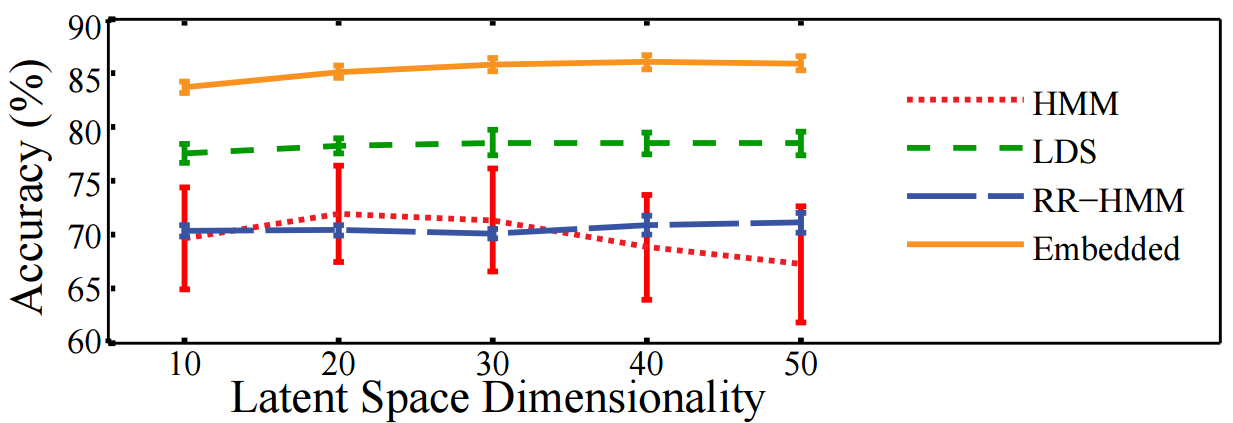
\includegraphics[scale=0.2]{audio_classification.png}  
    \caption{Accuracies and 95 \% confidence intervals for Human
vs. Non-human audio event classification, comparing
embedded HMMs to other common sequential models at
different latent state space sizes. (Fig adapted from \cite{ref20})}
    \label{fig:audio}
\end{figure}

An audio classification
task was performed using the data presented in \cite{ref26}.

The data consisted of sequences of 13-dimensional MelFrequency Cepstral Coefficients (MFCC) obtained
from short clips of raw audio data recorded using
a portable sensor device. Six classes of labeled audio
clips were present in the data, one being Human
Speech. 
For the experiment the latter five
classes were grouped into a single class of Non-human sounds to formulate a binary Human vs. Non-human classification
task. 

For each of the two classes embedded
HMMs were trained with 10, 20, ... , 50 latent dimensions using spectral learning and Gaussian RBF kernels with
bandwidth set with the ‘median trick’ and regularization
parameter $ \lambda = {10}^{-1}$.

For comparison, regular HMMs with
axis-aligned Gaussian observation models, LDSs and
RR-HMMs were trained using multi-restart EM (to
avoid local minima), stable Subspace ID and the spectral
algorithm of \cite{ref7} respectively, also
with 10, ... , 50 latent dimensions or states.

The mean accuracy and 95\% confidence intervals over
these 50 randomizations are shown in Figure \ref{fig:audio}. The
graph indicates that embedded HMMs have higher accuracy
and lower variance than other standard alternatives
at every model size. Though other learning
algorithms for HMMs and LDSs exist, this experiment
shows this to be a non-trivial sequence classification
problem where embedded HMMs significantly outperform
commonly used sequential models trained using
typical learning and model selection methods.

\subsection{Conclusion and Future work}

We have seen that how the limitations of local search techniques such as EM algorithm has motivated researchers to look into different waters for an alternate  solution. We saw how Hsu et al. \cite{ref2} showed that discrete HMMs can be learned
efficiently using spectral methods, under certain conditions. They built upon the idea that any HMM can be completely characterised
in terms of quantities that depend entirely on the observations, called the observable representation,
which can be estimated from data. Siddiqi et al. \cite{ref7} showed that the same algorithm works under slightly more general assumptions. Anandkumar et al. \cite{ref6} proposed a spectral algorithm for estimating more general latent variable models with parametric observations via a moment matching technique. And, building upon these works, we saw how Song et al.\cite{ref20} showed that these algorithms could be extended to kernel based methods with promising results.


However, when it comes to observations that are non parametric, very little work has been done on estimating latent variable models, including HMMs.

A commonly used heuristic is the nonparametric EM \cite{ref28}, which lacks theoretical underpinnings. This should not be surprising because EM is degenerate for most
nonparametric problems as a maximum likelihood procedure \cite{ref29}.

Although Siddiqi et al.\cite{ref7} proposed a heuristic based on kernel smoothing to modify the discrete algorithm for continuous observations, their procedure cannot be used to recover the joint or conditional probabilities
of a sequence, which would be needed to compute probabilities of events and other inference tasks.


While Song et al.'s \cite{ref20} procedure for estimating the Hilbert space embedding of an HMM provide theoretical guarantees, their bounds are in terms of \textit{reproducing kernel Hilbert Space}(RKHS) distance of the true and estimated embeddings. This metric depends on the choice of the kernel and it is not clear how it translates to a suitable distance measure on the observation space such as an L1 or L2 distance\cite{ref27}.

While their method can be used for prediction and pairwise testing, it still falls behind when it comes to recovering the joint and conditional densities. 



As real world distributions can be arbitrary, assuming parametric forms for the emission densities can be often too restrictive. Also, it is important to keep in mind that parametric models may introduce incongruous biases that cannot be reduced even with large datasets. 

Given all these scenarios,there is a fairly big scope for non-parametric models (including HMMs).

Recently, Kandasamy et al. \cite{ref27} have come up with nonparametric HMMs (using spectral algorithms) only assuming some mild smoothness conditions on the emission densities and have managed to extend the existing spectral methods for discrete HMMs to the continuous nonparametric setting. In doing so not only have they been able to recover the
joint/conditional densities, the theoretical results are in terms of more interpretable metrics, the
method outperforms baselines and is orders of magnitude faster to train.

The concern with this method, however, comes when it is extended to the practical setting.

For a one dimensional setting, there are numerical methods that can perform various c/q- matrix operations needed by this method using Chebyshev polynomials.

However, when it comes to multidimensional case, there is still a challenge to develop efficient procedures for these operations. 
With recent resurgence in interest in these spectral methods, it wouldn't be an overstatement to say that the solution is not that far into the future, and to know that a solution is somewhere there in the future can be a good motivation for anyone to wake up every morning excited about what the future holds. 



